% vim: syntax=tex:
\section{Topic}

Increasingly, \Glspl{gpu} are being used for general purpose computation
(\gls{gpgpu}). They have significantly altered the way high-performance
computing tasks can be performed today. To accelerate general-purpose
scientific applications, computationally intensive portions of the application
are passed to \glspl{gpu}. Once the \gls{gpu} has completed its task it sends
the result back to the \Gls{cpu} where the application code is running. This
process can make applications run noticeably faster.

Scientific applications require a large number of floating point number
operations, \Glspl{cpu} are not sufficient to carry out such computationally
intensive tasks. \glspl{cpu} are responsible for prioritization and execution
of every instruction. Generally, a processor is described by the number of
execution cores it owns. Modern \glspl{cpu} have eight cores while \Glspl{gpu}
have hundreds or more cores. More cores grant \glspl{gpu} the ability to
perform more tasks at the same time.

In computer architecture there are two main ways of processing: serial and
parallel. \Glspl{cpu} consist of a small number of cores (microprocessors) that
are best at processing serial data. On the other hand, \glspl{gpu} consist of
thousands of cores that are designed for processing parallel data. Given a
program, we can run the parallel portions of the code on \glspl{gpu} while the
serial portions run on the \gls{cpu}\@. The programmable \gls{gpu} has evolved
into a highly parallel, multithreaded, many core processor with tremendous
computational power. \Gls{cuda} is an architecture for utilizing and
distributing computational tasks onto a computer's \glspl{gpu}. As a parallel
computing platform and programming model, \gls{cuda} utilizes the power of
\gls{gpu} to achieve dramatic increases in computing performance
\cite{website:cudaCProgrammingGuide}. This fact is well illustrated in
\cref{fig:flops_gpu_vs_cpu}.

\begin{figure}[htb]
\centering
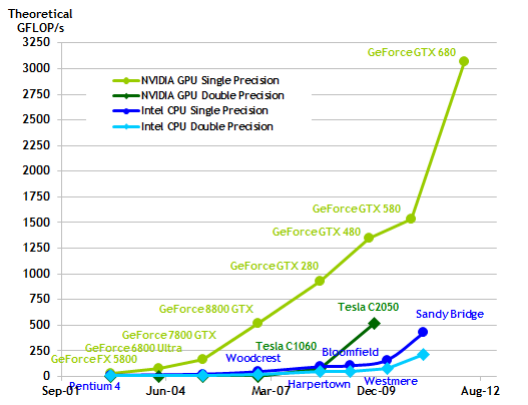
\includegraphics[scale=0.75]{img/floatingPoint.png}
\caption{Floating-Point Operations per Second for the \gls{cpu} and
         \gls{gpu} \cite{website:cudaCProgrammingGuide}}
\label{fig:flops_gpu_vs_cpu}
\end{figure}

Today, more than one million \gls{cuda}-enabled \glspl{gpu} are used by
software developers, scientists and researchers in order to obtained a large
performance gain in wide-ranging applications
\cite{website:cudaCProgrammingGuide}. A major challenge remains in being
able to seamlessly integrate multiple workstations to further parallelize the
computational tasks \cite{hadri2010identifying} \cite{hindman2009common}.
Current approaches provide the ability to parallelize tasks, but they are less
focused on optimally utilizing the varied capabilities of heterogeneous
graphics cards in a cluster of workstations (across many computer nodes).

We propose to create a framework for using both \Gls{mpi} and \gls{cuda} on a
cluster of computers to dynamically and easily assign computationally intensive
tasks to the machines participating in the cluster. \Gls{mpi} is a popularly
used standardized interface for communication among a group of computers. It
facilitates the passing of messages between the nodes in the cluster.

Our framework will be easy to use on a heterogeneous cluster of computers, each
containing a \Gls{cuda}-capable \gls{gpu}\@. The framework will optimize the
scheduling of low-level computational tasks based on the capabilities of the
varied \glspl{gpu} in the cluster. The framework will provide the system
administrator with the ability to easily configure it to allow optimal use of
the individual \glspl{gpu}. Overall, the goal is to create a framework that is
simple and easy to use, facilitating the combination of two powerful means of
computing to further increase the throughput and overall computing power of a
cluster.

We plan to evaluate the efficacy of our framework on the problem of vessel
extraction. Currently, we use a single \gls{gpu} to extract vascular structures
from a CT angiography scan which is computationally intensive
\cite{erdt2008automatic}. Using the framework to accelerate the computational
task will provide us with key insights on its usability.
